\documentclass[11pt,a4paper]{article}
\usepackage[a4paper,top=2.4cm,bottom=2.4cm,left=2.7cm,right=2.7cm]{geometry}
\usepackage[T5]{fontenc}
\usepackage[utf8]{inputenc}
\usepackage[vietnamese]{babel}
\usepackage{lmodern}
\usepackage{amsmath,amssymb,booktabs,array,graphicx,microtype,siunitx}
\usepackage{setspace,titlesec,fancyhdr,float}
\usepackage[hidelinks]{hyperref}
\graphicspath{{reports/figures/}{figures/}}
\sisetup{output-decimal-marker={,}}
\setstretch{1.15}
\setlength{\parindent}{0pt}
\setlength{\parskip}{6pt plus 1pt minus 1pt}
\renewcommand{\arraystretch}{1.16}
\titleformat{\section}{\large\bfseries}{\thesection.}{0.6em}{}
\titleformat{\subsection}{\normalsize\bfseries}{\thesubsection.}{0.6em}{}
\pagestyle{fancy}
\fancyhf{}
\fancyhead[L]{\small Uncertainty-aware DINOv3 Retrieval}
\fancyhead[R]{\small E1, E2A và E2B}
\fancyfoot[C]{\thepage}
\renewcommand{\headrulewidth}{0.4pt}
\renewcommand{\abstractname}{Tóm tắt}

\title{\bfseries\LARGE So sánh độ bất định theo ảnh và độ tin cậy theo cặp\\[0.3em]
trong truy hồi ảnh với DINOv3}
\author{Báo cáo tổng hợp thực nghiệm E1, E2A và E2B}
\date{18 tháng 9 năm 2026}

\begin{document}
\maketitle
\thispagestyle{plain}

\begin{abstract}
Báo cáo tổng hợp chuỗi thực nghiệm E1--E2A--E2B cho truy hồi ảnh trên
CUB-200-2011. E1 gán một uncertainty score cho từng ảnh và dùng score này để
sắp lại Top-$N$. E2B học Pairwise Confidence trực tiếp cho từng cặp ảnh truy
vấn--ứng viên, sau đó đánh giá riêng confidence và phép kết hợp với cosine.
Giữa hai bước này, E2A so sánh bốn cách tạo embedding và chọn M1 final CLS làm
representation chung cho E2B. Mọi so sánh E2B dùng cùng embedding M1, cùng
danh sách ứng viên và $N\in\{10,20,50,100\}$.

Kết quả cho thấy Image Uncertainty không phù hợp để thay thế thứ tự cosine:
ở E1, Recall@1 giảm từ \SI{87.9980}{\percent} xuống
$\SI{79.8447}{\percent}\pm\SI{0.2108}{\percent}$ tại $N=10$ và còn
\SI{27.2676}{\percent} tại $N=100$. Trong phép so sánh E2B dùng cùng tập train,
Pairwise Confidence luôn tốt hơn Image Uncertainty nhưng vẫn thấp hơn
baseline. Fusion với $\lambda=0{,}75$ giữ nguyên Recall@1
\SI{88.0149}{\percent}, đồng thời tăng nhẹ Recall@2/4/8. Các khoảng bootstrap
95\% đều chứa 0, vì vậy chưa có bằng chứng rằng Fusion cải thiện Recall@1.

\textbf{Từ khóa:} DINOv3, truy hồi ảnh, uncertainty, pairwise confidence,
reranking.
\end{abstract}

\section{Mục tiêu}
Chuỗi thực nghiệm trả lời ba câu hỏi liên tiếp:
\begin{enumerate}
  \item Uncertainty của một ảnh có thể dùng để sắp lại kết quả cosine hay không?
  \item Cách tạo embedding nào từ CLS Token và Patch Tokens của DINOv3 phù hợp
  nhất để làm representation chung cho các bước truy hồi tiếp theo?
  \item Nếu uncertainty theo ảnh không hiệu quả, confidence học trực tiếp trên
  một cặp ảnh có cung cấp tín hiệu phù hợp hơn cho truy hồi hay không?
\end{enumerate}

E1, E2A và E2B đều giữ nguyên backbone DINOv3. E1 chạy ba seed để đo mức biến
động của EDL head. M3, M4 và E2B chỉ chạy seed 42, vì vậy các kết quả này được
báo cáo theo một lần chạy và không trình bày mean $\pm$ std.

\section{Phương pháp}
\subsection{Ký hiệu chung}
Tập dữ liệu được ký hiệu là
$\mathcal{D}=\{(x_i,y_i)\}_{i=1}^{M}$, trong đó $x_i$ là ảnh thứ $i$,
$y_i$ là nhãn lớp và $M$ là số ảnh. Chỉ số $c\in\{1,\ldots,C\}$ biểu diễn
lớp, $t\in\{1,\ldots,T\}$ biểu diễn Patch Token, $K$ là ngưỡng của
Recall@$K$, còn $N$ là số ứng viên đầu được sắp lại. Quy ước này tách rõ
$C=100$ lớp trong mỗi nửa CUB, $T=196$ Patch Tokens và
$N\in\{10,20,50,100\}$.

Vector được in đậm. $\mathbf z_i$ là embedding thô của $x_i$ và
$\widehat{\mathbf z}_i=\mathbf z_i/\lVert\mathbf z_i\rVert_2$ là embedding
đã chuẩn hóa L2. Với query $x_i$ và candidate $x_j$, cosine similarity là
\begin{equation}
 s^{\mathrm{cos}}_{ij}
 =\widehat{\mathbf z}_i^{\top}\widehat{\mathbf z}_j.
\end{equation}

\subsection{DINOv3 Baseline}
Với ảnh $x_i$, final CLS token $\mathbf h_i^{\mathrm{cls}}$ được dùng làm
embedding thô rồi chuẩn hóa L2:
\begin{equation}
 \mathbf z_i=\mathbf h_i^{\mathrm{cls}},\qquad
 \widehat{\mathbf z}_i=\frac{\mathbf z_i}{\lVert\mathbf z_i\rVert_2},
 \qquad s^{\mathrm{cos}}_{ij}
 =\widehat{\mathbf z}_i^\top\widehat{\mathbf z}_j.
\end{equation}
Gallery được xếp theo cosine giảm dần và loại chính ảnh truy vấn. Đây là R0
trong E1 và DINOv3 Baseline trong E2B.

\subsection{Bốn phương pháp tạo embedding trong E2A}
Với ảnh $x_i$, lớp cuối của DINOv3 tạo CLS Token
$\mathbf h_i^{\mathrm{cls}}\in\mathbb{R}^{768}$ và $T=196$ Patch Tokens
$\mathbf h_{it}^{\mathrm{patch}}\in\mathbb{R}^{768}$. Bốn phương pháp E2A
khác nhau ở cách chuyển các token này thành
$\mathbf z_i^{(m)}\in\mathbb{R}^{768}$. Sau đó mọi phương pháp
đều chuẩn hóa L2 và dùng cùng cosine similarity:
\begin{equation}
 \widehat{\mathbf z}_i^{(m)}
 =\frac{\mathbf z_i^{(m)}}{\lVert\mathbf z_i^{(m)}\rVert_2},
 \qquad s_{ij}^{(m)}
 =(\widehat{\mathbf z}_i^{(m)})^\top\widehat{\mathbf z}_j^{(m)}.
\end{equation}

\paragraph{M1 --- CLS Token.}
M1 dùng trực tiếp token tổng hợp sẵn của DINOv3:
\begin{equation}
 \mathbf z_i^{(1)}=\mathbf h_i^{\mathrm{cls}}.
\end{equation}
M1 không có tham số cần train. Đây cũng là embedding của DINOv3 Baseline.

\paragraph{M2 --- Mean Patch Pooling.}
M2 lấy trung bình 196 Patch Tokens:
\begin{equation}
 \overline{\mathbf h}_i^{\mathrm{patch}}
 =\frac{1}{T}\sum_{t=1}^{T}\mathbf h_{it}^{\mathrm{patch}},
 \qquad \mathbf z_i^{(2)}=\overline{\mathbf h}_i^{\mathrm{patch}}.
\end{equation}
M2 không cần train. Bốn Register Tokens và CLS Token không tham gia phép lấy
trung bình, vì vậy mọi vùng ảnh đóng góp với trọng số bằng nhau.

\paragraph{M3 --- CLS + Mean Patch Fusion.}
M3 ghép CLS Token với Mean Patch thành vector 1.536 chiều, rồi học một phép
chiếu tuyến tính về 768 chiều:
\begin{equation}
 \mathbf z_i^{(3)}
 =\mathbf W[\mathbf h_i^{\mathrm{cls}};
 \overline{\mathbf h}_i^{\mathrm{patch}}]+\mathbf b,
 \qquad \mathbf W\in\mathbb{R}^{768\times1536}.
\end{equation}
Chỉ $\mathbf W$ và $\mathbf b$ được train bằng Proxy Anchor; backbone DINOv3 được giữ nguyên.
M3 kiểm tra liệu kết hợp thông tin toàn ảnh từ CLS với thông tin vùng ảnh từ
Patch Tokens có tốt hơn dùng riêng CLS hay không.

\paragraph{M4 --- Attention Pooling.}
M4 học một điểm cho từng Patch Token, chuyển các điểm thành trọng số bằng
softmax rồi tính tổng có trọng số:
\begin{align}
 r_{it}&=\mathbf w_2^\top\tanh(
 \mathbf W_1\mathbf h_{it}^{\mathrm{patch}}+\mathbf b_1)+b_2,\\
 a_{it}&=\frac{\exp(r_{it})}{\sum_{\tau=1}^{T}\exp(r_{i\tau})},\\
 \mathbf z_i^{(4)}&=\sum_{t=1}^{T}a_{it}\mathbf h_{it}^{\mathrm{patch}}.
\end{align}
Mạng tính trọng số có kích thước $768\rightarrow256\rightarrow1$ và được
train bằng Proxy Anchor; DINOv3 vẫn được giữ nguyên. M4 học mức đóng góp của
từng Patch Token vào embedding chung. Các trọng số $a_{it}$ chỉ dùng để hỗ trợ
phân tích, không được diễn giải là bằng chứng mô hình đã xác định đúng vị trí
con chim.

\subsection{Image Uncertainty}
EDL head nhận CLS feature 768 chiều của ảnh $x_i$ và sinh evidence,
tham số Dirichlet và uncertainty:
\begin{equation}
 e_{ic}=\operatorname{softplus}([f_{\theta}(x_i)]_c),\qquad
 \alpha_{ic}=e_{ic}+1,\qquad
 S_i=\sum_{c=1}^{C}\alpha_{ic},\qquad
 u_i=\frac{C}{S_i},\quad C=100.
\end{equation}
Image Uncertainty Reranking giữ nguyên tập ứng viên cosine, chỉ sắp lại $N$ ảnh
đầu theo $u_j$ tăng dần. Các ảnh ngoài Top-$N$ không được đưa lên trên.

\subsection{Evidential Embedding}
Nhánh này dùng trực tiếp vector tham số Dirichlet
$\boldsymbol\alpha_i=(\alpha_{i1},\ldots,\alpha_{iC})$ và khoảng cách L2:
\begin{equation}
 d^{\alpha}_{ij}=\lVert\boldsymbol\alpha_i-\boldsymbol\alpha_j\rVert_2.
\end{equation}
Cách biểu diễn này dựa trên Evidential Transformers, nhưng backbone được thay
bằng DINOv3 nên được xem là một adaptation, không phải tái lập nguyên bản.

\subsection{Pairwise Confidence và Fusion}
Mạng MLP nhận hai embedding theo thứ tự cố định query trước, candidate sau:
\begin{align}
 \boldsymbol\phi_{ij}
 &=[\widehat{\mathbf z}_i;\widehat{\mathbf z}_j;
 |\widehat{\mathbf z}_i-\widehat{\mathbf z}_j|],\\
 \ell_{ij}&=g_{\omega}(\boldsymbol\phi_{ij}),\qquad
 c_{ij}=\sigma(\ell_{ij}).
\end{align}
MLP có kiến trúc $2304\rightarrow512\rightarrow128\rightarrow1$, ReLU và
dropout 0,1. Mạng được train bằng Binary Cross Entropy trên số positive và
negative pairs bằng nhau. Negative gần nhất được lấy một lần từ cosine
Top-100 trên fit set và không cập nhật online.

Fusion dùng điểm
\begin{equation}
 s^{\mathrm{final}}_{ij}(\lambda)
 =\lambda s^{\mathrm{cos}}_{ij}+(1-\lambda)c_{ij}.
\end{equation}
Các giá trị $\lambda\in\{0;0{,}25;0{,}5;0{,}75;0{,}9;1\}$ đều được lưu.
$\lambda=0$ là Pairwise Confidence, còn $\lambda=1$ tái tạo baseline.

\section{Thiết lập thực nghiệm}
\subsection{Dữ liệu và môi trường thực thi}
CUB-200-2011 gồm 11.788 ảnh. Classes 0--99 tạo tập development 5.864 ảnh;
classes 100--199 tạo tập test 5.924 ảnh chưa xuất hiện khi train. Development
được chia theo từng lớp thành 4.687 ảnh fit và 1.177 ảnh validation với seed
chia dữ liệu cố định bằng 42.

Backbone là \texttt{facebook/dinov3-vitb16-pretrain-lvd1689m}, ảnh đầu vào
$224\times224$. Thực nghiệm chạy bằng Python 3.12.13, PyTorch 2.10.0,
CUDA 12.8 và hai Tesla T4. Backbone được giữ nguyên trong toàn bộ chuỗi thực
nghiệm; chỉ các head hoặc lớp tổng hợp được train ở những nhánh tương ứng.

\subsection{Đánh giá truy hồi}
Tất cả phương pháp dùng cùng quy tắc loại chính ảnh truy vấn khỏi gallery.
Với tập $\mathcal{Q}$ gồm các query, đặt
$h_i^{(K)}=1$ nếu Top-$K$ của query $x_i$ chứa ít nhất một ảnh cùng lớp và
bằng 0 trong trường hợp ngược lại. Khi đó
\begin{equation}
 \operatorname{Recall@}K
 =\frac{1}{|\mathcal Q|}\sum_{x_i\in\mathcal Q}h_i^{(K)},
 \qquad H@K=\sum_{x_i\in\mathcal Q}h_i^{(K)}.
\end{equation}
$H@K$ là số query truy hồi thành công, được gọi là Hits@$K$ trong phần chọn
mô hình; đây là số đếm tương ứng với Recall@$K$, không phải một metric khác.
Các kết quả được báo cáo tại $K\in\{1,2,4,8\}$.

\subsection{Protocol E1 và E2A}
Trong E1, ba seed 42, 43 và 44 dùng cùng một fit/validation split. Epoch và
$N$ được chọn trên validation; sau đó EDL head được train lại trên toàn bộ
development để đánh giá test. Trong E2A, M3 và M4 được train trên classes
0--99, chọn checkpoint bằng validation rồi mới đánh giá cùng M1 và M2 trên
classes 100--199.

\subsection{Tạo dữ liệu và train E2B}
Đầu tiên, mỗi ảnh fit được dùng làm query để lấy Top-100 candidate gần nhất
theo cosine M1. Chính ảnh query được loại bỏ. Candidate list này được tạo một
lần và giữ cố định, nên hard-negative mining không thay đổi theo MLP đang
train.

Ở mỗi epoch, một query tạo 32 cặp: 16 positive cùng lớp, 8 hard negative khác
lớp lấy từ Top-100 và 8 negative khác lớp được chọn ngẫu nhiên. Toàn bộ 4.687
query tạo 149.984 cặp, với số positive và negative bằng nhau. Hai đầu của cặp
được đổi vị trí ngẫu nhiên với xác suất 50\% rồi xáo trộn trước khi train bằng
Binary Cross Entropy. Các cặp được lấy mẫu lại một cách xác định ở mỗi epoch
từ seed gốc 42; random swap chỉ là tăng cường dữ liệu khi train.

Validation và test không dùng phân bố cân bằng này. MLP chấm toàn bộ Top-100
cosine theo đúng thứ tự query--candidate; nhãn bằng 1 nếu hai ảnh cùng lớp và
bằng 0 nếu khác lớp. Do đó validation có
$1.177\times100=117.700$ cặp để chọn checkpoint bằng BCE, còn test có
$5.924\times100=592.400$ cặp để tính confidence và đánh giá reranking.

EDL control và Pairwise Confidence đều chỉ train trên 4.687 ảnh fit để bảo
đảm so sánh cùng dữ liệu. Checkpoint Pairwise Confidence được chọn tại epoch
19 theo validation BCE. Trên validation với $N=100$, $\lambda=0{,}75$ được
chọn theo thứ tự Hits@1 $\rightarrow$ Hits@2 $\rightarrow$ Hits@4
$\rightarrow$ Hits@8 $\rightarrow$ $\lambda$ lớn hơn.

\section{Kết quả E1: uncertainty theo ảnh}
\subsection{Kết quả chính}
\begin{table}[H]
\centering
\caption{Recall@K trên test, mean $\pm$ sample standard deviation qua ba seed
(\%). R1 dùng $N=10$ được chọn trên validation.}
\begin{tabular}{@{}lrrrr@{}}
\toprule
Phương pháp & R@1 & R@2 & R@4 & R@8\\ \midrule
R0: DINOv3 cosine & 87,9980 & 92,7583 & 95,2566 & 97,0122\\
R1: Image Uncertainty
& $79,8447\pm0,2108$ & $88,3075\pm0,2000$
& $93,9849\pm0,0639$ & $96,8490\pm0,0195$\\
\bottomrule
\end{tabular}
\end{table}

R1 giảm trung bình 8,1533 điểm phần trăm tại R@1. Paired bootstrap 95\% của
R@1 hoàn toàn dưới 0 ở cả ba seed: $[-8{,}9129;-6{,}9379]$,
$[-9{,}1661;-7{,}2586]$ và $[-9{,}3180;-7{,}3430]$ điểm phần trăm. Kết quả
không hỗ trợ giả thuyết rằng uncertainty theo ảnh cải thiện thứ hạng cosine.

\subsection{Ảnh hưởng của Top-$N$}
\begin{table}[H]
\centering
\caption{Image Uncertainty theo Top-$N$ trên test, trung bình ba seed (\%).}
\begin{tabular}{@{}crrrr@{}}
\toprule
$N$ & R@1 & R@2 & R@4 & R@8\\ \midrule
10  & 79,8447 & 88,3075 & 93,9849 & 96,8490\\
20  & 72,5073 & 83,1702 & 91,2953 & 96,0556\\
50  & 51,1591 & 64,3991 & 78,8375 & 90,3050\\
100 & 27,2676 & 38,7857 & 53,8431 & 70,6842\\
\bottomrule
\end{tabular}
\end{table}

Khi $N$ tăng, nhiều ảnh vốn được cosine đặt đúng bị đưa xuống dưới. Vì vậy
$N=10$ là lựa chọn ít bất lợi nhất, không phải một cấu hình vượt baseline.

\section{Kết quả E2A: chọn representation cho E2B}
Mục tiêu của E2A là chọn một representation chung trước khi thực hiện E2B.
Bốn phương pháp M1--M4 được so sánh bằng cùng cosine similarity, quy tắc loại
self-match và Recall@K. M1/M2 dùng trực tiếp feature DINOv3; M3/M4 được train
trên classes 0--99 với seed 42 và chọn checkpoint bằng validation. Sau đó cả
bốn phương pháp được đánh giá trên 5.924 ảnh thuộc classes 100--199.

\begin{table}[H]
\centering
\caption{So sánh bốn representation pipelines của E2A trên classes 100--199
(\%). Kết quả tốt nhất tại từng Recall được in đậm.}
\label{tab:e2a-representations}
\begin{tabular}{@{}llrrrr@{}}
\toprule
Mã & Representation & R@1 & R@2 & R@4 & R@8\\ \midrule
M1 & CLS Token & \textbf{88,0149} & \textbf{92,7583}
& \textbf{95,2566} & \textbf{97,0122}\\
M2 & Mean Patch Pooling & 45,7461 & 57,8663 & 68,2309 & 78,7643\\
M3 & CLS + Mean Patch Fusion & 87,2890 & 92,2687 & \textbf{95,2566} & 96,8771\\
M4 & Attention Pooling & 80,6550 & 88,3693 & 92,8258 & 95,9149\\
\bottomrule
\end{tabular}
\end{table}

M1 đạt Recall@1 cao nhất với 5.214 query thành công, nhiều hơn M3 43 query.
Tiêu chí đầu tiên vì vậy đã đủ để chọn M1 mà không cần dùng các bước phân xử
Hits@2, Hits@4, Hits@8, số tham số và thứ tự M1--M4. M1 cũng không cần train
thêm và chính là DINOv3 cosine baseline. E2B do đó cố định đầu vào là final CLS
Token của M1 sau chuẩn hóa L2; embedding không thay đổi khi train Pairwise
Confidence.

\section{Kết quả E2B: confidence theo cặp}
Sau khi cố định representation M1, E2B so sánh năm cách xếp hạng trên cùng
candidate list. Phần đầu báo cáo kết quả tại $N=100$; các phần sau lần lượt
phân tích ảnh hưởng của $N$ và hệ số $\lambda$.

\subsection{So sánh năm phương pháp}
\begin{table}[H]
\centering
\caption{Kết quả trên 5.924 test queries (\%). Ba phương pháp reranking dùng
cùng $N=100$; EDL control và Pairwise Confidence cùng train trên fit set.}
\begin{tabular}{@{}lrrrr@{}}
\toprule
Phương pháp & R@1 & R@2 & R@4 & R@8\\ \midrule
DINOv3 Baseline & \textbf{88,0149} & 92,7583 & 95,2566 & 97,0122\\
Evidential Embedding & 34,4868 & 44,9021 & 55,6550 & 66,4078\\
Image Uncertainty & 27,3801 & 41,3403 & 57,1911 & 73,8521\\
Pairwise Confidence & 78,9163 & 88,6563 & 93,8049 & 96,5057\\
Fusion ($\lambda=0{,}75$) & \textbf{88,0149} & \textbf{92,7920}
& \textbf{95,3410} & \textbf{97,0459}\\
\bottomrule
\end{tabular}
\end{table}

Fusion giữ nguyên 5.214 Hits@1 như baseline. R@2 tăng 2 query, R@4 tăng 5
query và R@8 tăng 2 query. Paired bootstrap 95\% của chênh lệch Fusion--baseline
lần lượt là $[-0{,}3038;0{,}3376]$, $[-0{,}2363;0{,}3038]$,
$[-0{,}1350;0{,}2870]$ và $[-0{,}1519;0{,}2194]$ điểm phần trăm. Tất cả đều
chứa 0, do đó các thay đổi nhỏ này chưa đủ để kết luận có cải thiện ổn định.

\subsection{So sánh công bằng theo Top-$N$}
\begin{table}[H]
\centering
\caption{Recall@1 theo cùng số ứng viên được sắp lại (\%). Fusion dùng
$\lambda=0{,}75$ đã chọn trên validation.}
\begin{tabular}{@{}crrr@{}}
\toprule
$N$ & Image Uncertainty & Pairwise Confidence & Fusion\\ \midrule
10  & 80,3174 & 84,7907 & 88,0149\\
20  & 73,5989 & 83,7779 & 88,0149\\
50  & 53,9669 & 81,2289 & 88,0149\\
100 & 27,3801 & 78,9163 & 88,0149\\
\bottomrule
\end{tabular}
\end{table}

Pairwise Confidence tốt hơn Image Uncertainty ở mọi $N$. Tuy nhiên, khi dùng
đơn lẻ, cả hai đều thấp hơn cosine baseline. Điều này cho thấy quan hệ giữa
query và candidate phù hợp với retrieval hơn uncertainty của candidate riêng
lẻ, nhưng confidence vẫn chưa đủ chính xác để thay hoàn toàn cosine.

\begin{figure}[H]
\centering
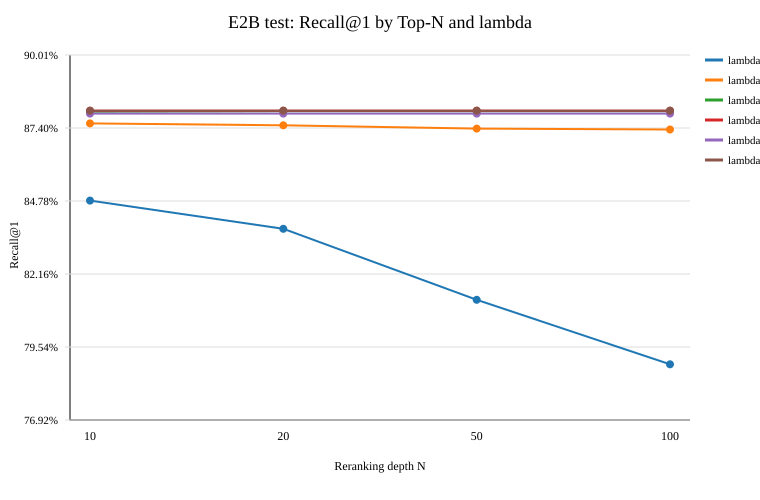
\includegraphics[width=0.88\textwidth]{e2b_topn_lambda_recall1.png}
\caption{Recall@1 của Fusion theo Top-$N$ và $\lambda$. $\lambda=0{,}75$ giữ
R@1 ngang baseline ở cả bốn $N$; các $\lambda$ nhỏ làm confidence chi phối và
giảm kết quả khi $N$ tăng.}
\label{fig:lambda-grid}
\end{figure}

\subsection{Ảnh hưởng của $\lambda$ tại $N=100$}
\begin{table}[H]
\centering
\caption{Fusion grid trên test tại $N=100$ (\%).}
\begin{tabular}{@{}crrrr@{}}
\toprule
$\lambda$ & R@1 & R@2 & R@4 & R@8\\ \midrule
0    & 78,9163 & 88,6563 & 93,8049 & 96,5057\\
0,25 & 87,3396 & 92,2687 & 95,3579 & 97,0966\\
0,50 & 87,9980 & 92,5219 & \textbf{95,4254} & 97,0966\\
0,75 & \textbf{88,0149} & \textbf{92,7920} & 95,3410 & 97,0459\\
0,90 & 87,9136 & 92,7076 & 95,3410 & 97,0797\\
1    & \textbf{88,0149} & 92,7583 & 95,2566 & 97,0122\\
\bottomrule
\end{tabular}
\end{table}

Kết quả tốt nhất không xuất hiện khi confidence đứng một mình. Confidence chỉ
hữu ích như một tín hiệu phụ có trọng số nhỏ bên cạnh cosine.

\section{Phân tích thay đổi Top-1 và failure cases}
% Trên toàn bộ 592.400 cặp ứng viên test, Pairwise Confidence đạt AUROC 0,7054,
% AUPRC 0,6365, Brier score 0,3646 và ECE 0,3689. Ở candidate cosine Top-1,
% AUROC là 0,6287 và ECE là 0,0833. Confidence có khả năng phân biệt nhất định
% nhưng chưa được hiệu chỉnh tốt trên toàn bộ Top-100; phần lớn score tập trung
% ở khoảng 0,9--1,0.

% \begin{figure}[H]
% \centering
% 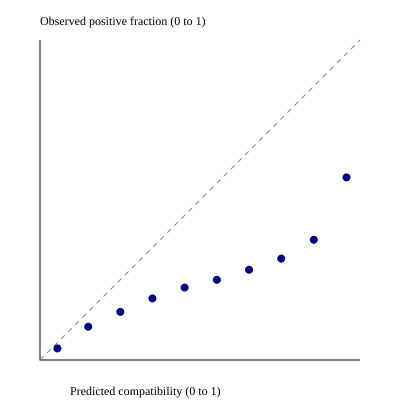
\includegraphics[width=0.55\textwidth]{e2b_candidate_calibration.png}
% \caption{Biểu đồ calibration của Pairwise Confidence trên các cặp ứng viên
% test. Đường đứt thể hiện trường hợp score khớp hoàn toàn tỉ lệ cặp cùng lớp.}
% \end{figure}

Để giải thích thay đổi Recall@1, mỗi query được phân loại theo việc Top-1 trước
và sau reranking đúng hay sai. Tại $N=100$, Image Uncertainty sửa đúng 134
query nhưng làm sai thêm 3.726
query. Pairwise Confidence sửa đúng 213 và làm sai 752 query. Fusion cân bằng
đúng 47 query được sửa và 47 query bị làm sai, nên tổng Hits@1 không đổi.

\begin{figure}[H]
\centering
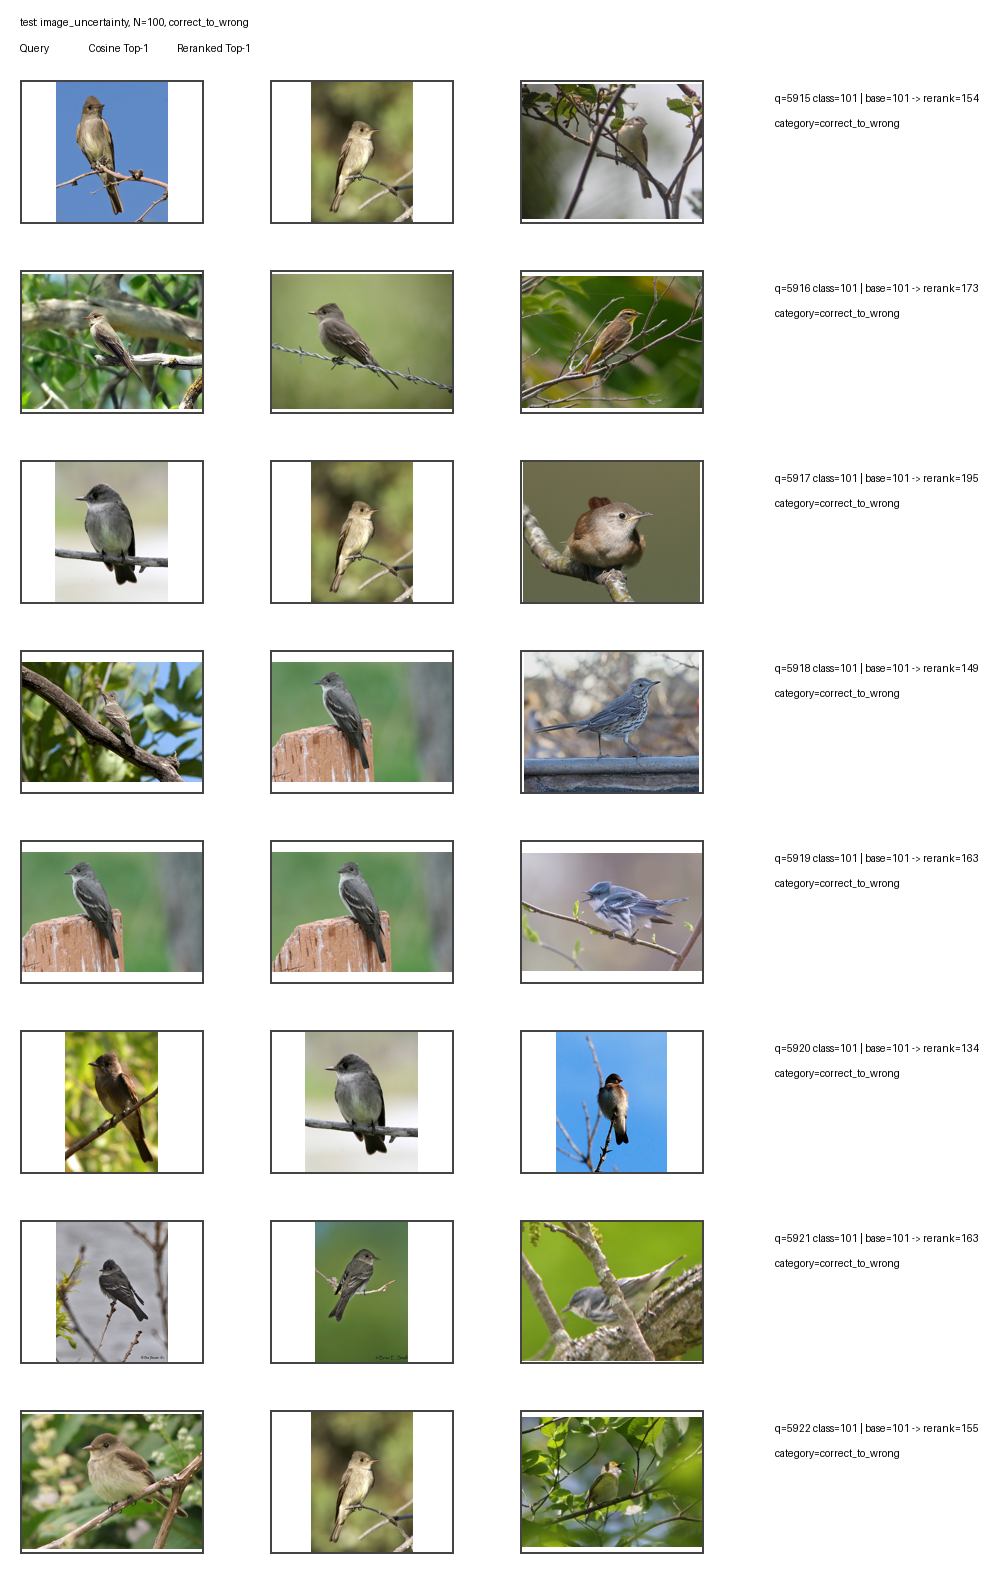
\includegraphics[width=0.92\textwidth]{image_uncertainty_correct_to_wrong.png}
\caption{Các trường hợp Image Uncertainty $N=100$ làm kết quả cosine đúng
thành sai. Cột trái là query, giữa là cosine Top-1, phải là kết quả sau rerank.}
\end{figure}

\begin{figure}[H]
\centering
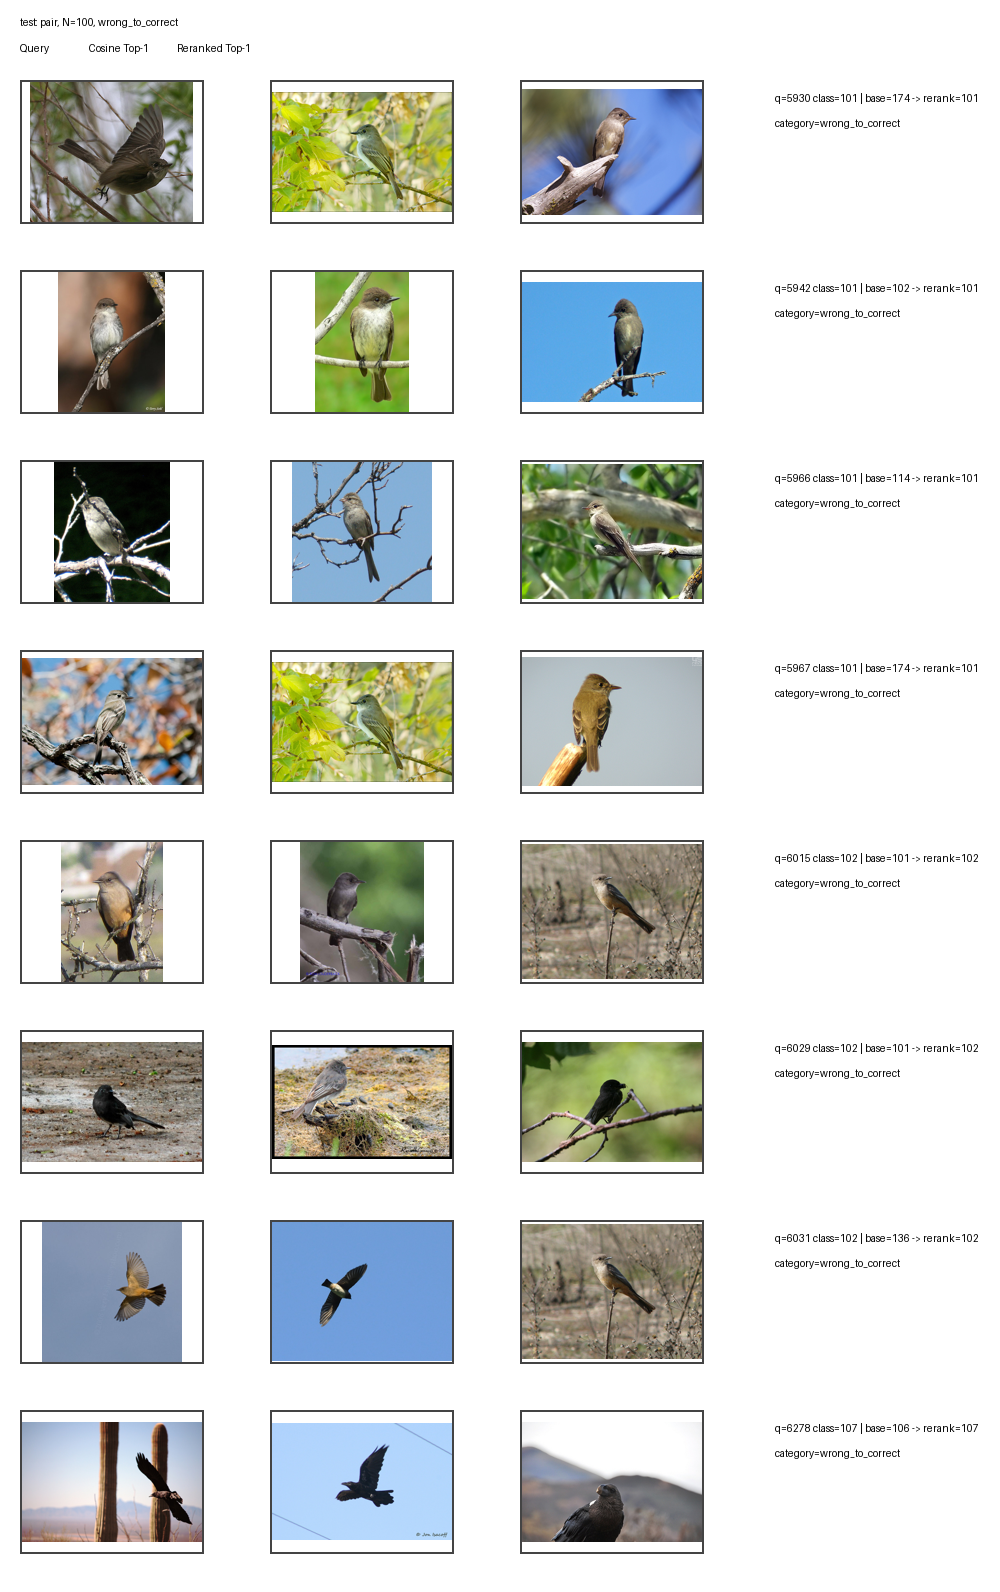
\includegraphics[width=0.92\textwidth]{pair_wrong_to_correct.png}
\caption{Các trường hợp Pairwise Confidence $N=100$ sửa kết quả cosine sai
thành đúng. Mô hình thường đưa lên ảnh có hình dáng và chi tiết loài gần query.}
\end{figure}

\begin{figure}[H]
\centering
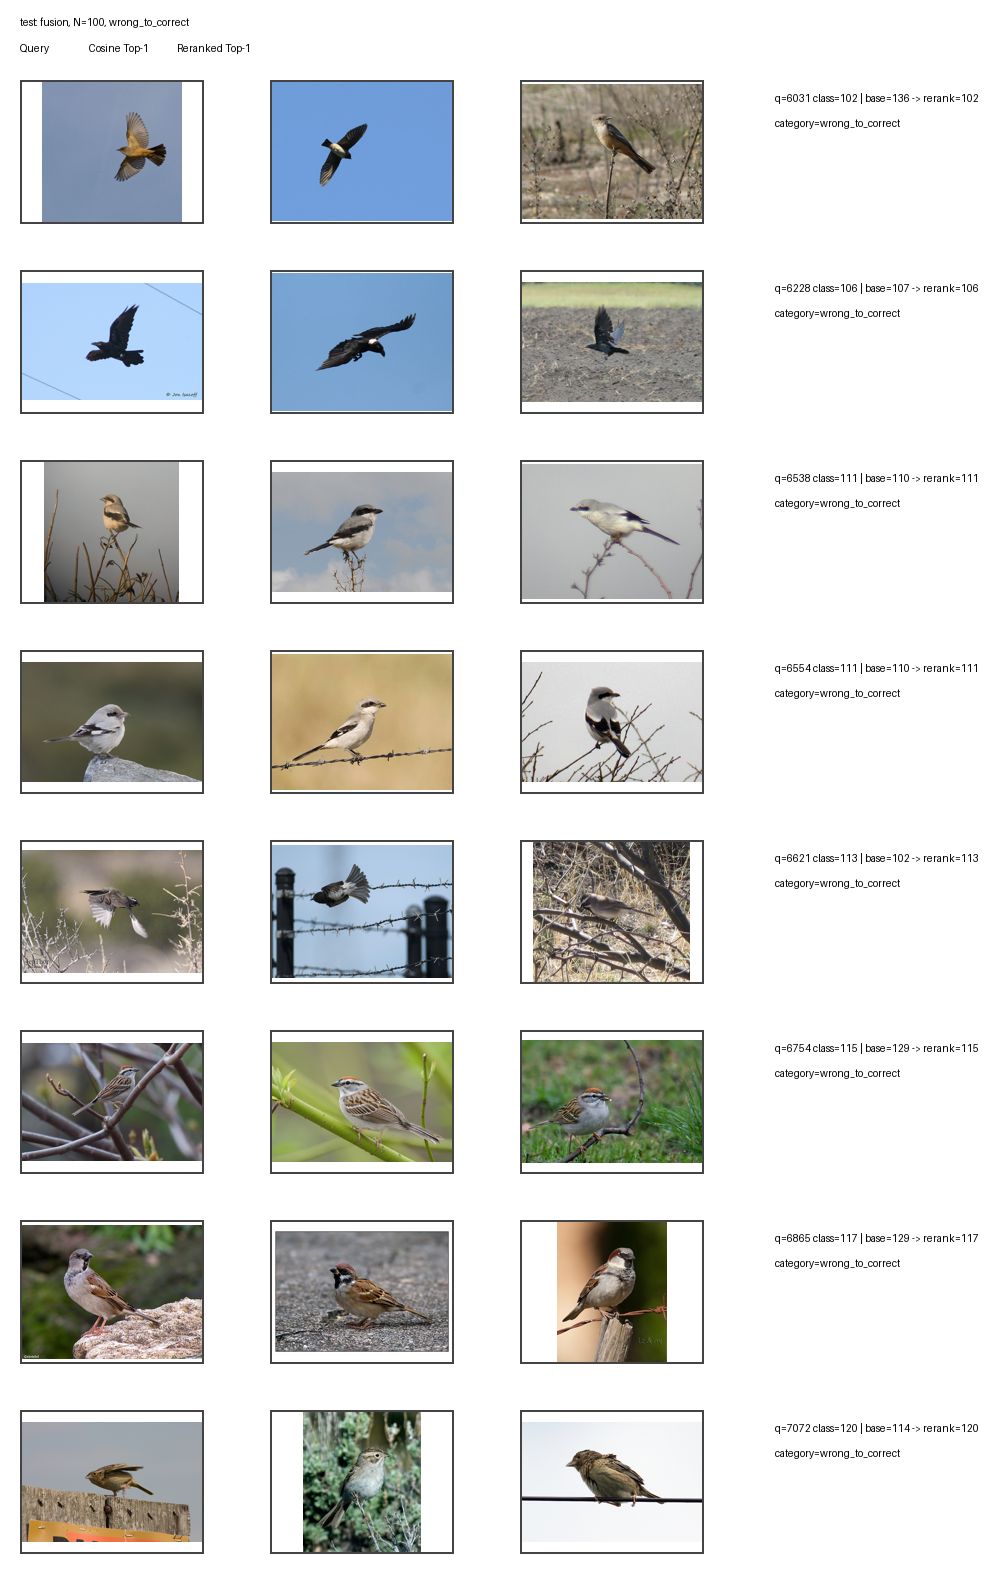
\includegraphics[width=0.92\textwidth]{fusion_wrong_to_correct.png}
\caption{Các trường hợp Fusion $N=100$, $\lambda=0{,}75$ sửa đúng Top-1.}
\end{figure}

\begin{figure}[H]
\centering
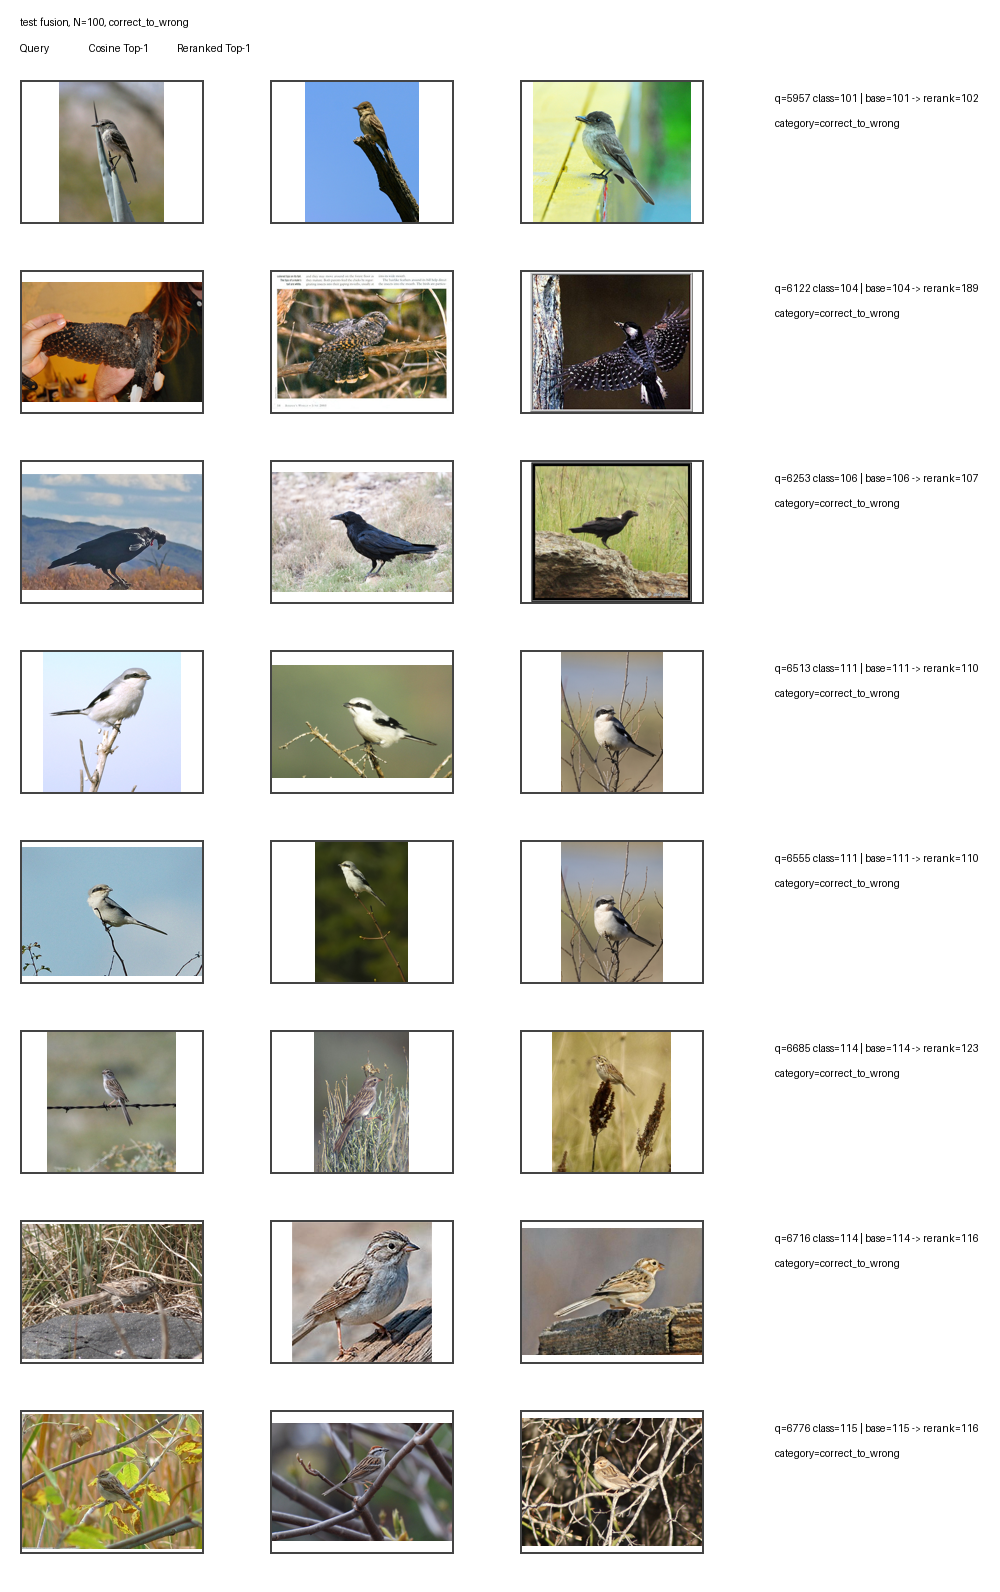
\includegraphics[width=0.92\textwidth]{fusion_correct_to_wrong.png}
\caption{Các trường hợp Fusion làm Top-1 đúng thành sai. Việc số trường hợp
sửa đúng và làm sai bằng nhau giải thích Recall@1 không thay đổi.}
\end{figure}

\section{Thảo luận}
\subsection{Từ uncertainty theo ảnh đến confidence theo cặp}
E1 và E2B cùng cho thấy uncertainty của một candidate không đo trực tiếp mức
phù hợp với một query cụ thể. Khi $N$ tăng, Image Uncertainty thay đổi nhiều
vị trí cosine đúng hơn và Recall giảm nhanh. Pairwise Confidence sử dụng đồng
thời query và candidate nên tốt hơn Image Uncertainty ở mọi $N$, nhưng vẫn
chưa đủ chính xác để thay cosine khi dùng riêng.

\subsection{Vai trò của representation và Fusion}
E2A chọn M1 vì final CLS Token đạt Recall@1 cao nhất. M3 không vượt M1 dù có
thêm lớp học được; M2 và M4 chỉ tổng hợp Patch Tokens và đều cho kết quả thấp
hơn.
Việc cố định M1 cho tất cả nhánh E2B giúp kết quả phản ánh cách dùng
uncertainty hoặc confidence, thay vì khác biệt do đầu vào.

Fusion hoạt động ổn định hơn vì vẫn đặt trọng số chính vào cosine. Tại
$\lambda=0{,}75$, confidence chỉ điều chỉnh thứ tự trong candidate list. R@2,
R@4 và R@8 tăng nhẹ, nhưng các khoảng bootstrap đều chứa 0; vì vậy chưa thể
kết luận Fusion tạo ra cải thiện ổn định so với baseline.

\subsection{Giới hạn của thực nghiệm}
E2B chỉ chạy một seed và classes 100--199 đã được dùng để chọn representation
trong E2A. Kết quả vì thế chưa phản ánh độ biến động giữa nhiều lần train và
không phải đánh giá trên một final test hoàn toàn độc lập. Bootstrap trong báo
cáo chỉ mô tả độ biến động theo query của benchmark hiện tại.

Baseline E1 có 5.213 Hits@1, còn baseline E2A/E2B có 5.214 Hits@1 vì hai
feature cache được trích xuất bởi hai pipeline riêng. Mỗi bảng vẫn so sánh các
phương pháp trên cùng cache và ranking, nên chênh lệch một query này không làm
thay đổi kết luận trong từng thực nghiệm.

\section{Kết luận}
E2A chọn M1 final CLS Token làm representation chung vì đạt Recall@1 cao nhất
trong bốn pipeline. Trên representation này, Image Uncertainty Reranking không
cải thiện truy hồi và suy giảm nhanh khi tăng Top-$N$. Pairwise Confidence
tốt hơn rõ rệt so với Image Uncertainty trong điều kiện cùng tập train và cùng
số ứng viên, nhưng chưa thể thay cosine.
Fusion với trọng số cosine lớn giữ nguyên R@1 và cải thiện rất nhỏ các Recall@K
còn lại. Hướng tiếp theo nên chạy E2B với nhiều seed, cải thiện confidence và
đánh giá trên một benchmark độc lập chưa từng dùng để chọn phương pháp.

\section*{Tài liệu tham khảo}
\begin{enumerate}
  \item A. Simeoni et al., \emph{DINOv3}, 2025.
  \href{https://arxiv.org/abs/2508.10104}{arXiv:2508.10104}.
  \item M. Sensoy, L. Kaplan, M. Kandemir, \emph{Evidential Deep Learning to
  Quantify Classification Uncertainty}, 2018.
  \href{https://arxiv.org/abs/1806.01768v3}{arXiv:1806.01768v3}.
  \item D. Đorđević, S. Kumar, \emph{Evidential Transformers for Improved
  Image Retrieval}, 2025.
  \href{https://arxiv.org/abs/2409.01082v2}{arXiv:2409.01082v2}.
  \item C. Wah et al., \emph{The Caltech-UCSD Birds-200-2011 Dataset}, 2011.
\end{enumerate}

\end{document}
